\section{Flüssigkristalle}
    Flüssigkristalle haben zwischen den Aggregatzuständen ``fest'' und ``flüssig'' einen weiteren Aggregatzustand. Der ``flüssigkristalline'' Aggregatzustand macht sich erkennbar durch die trübe Farbe.        

    Es wird in 3 verschiedene flüssigkristalline-Phasen unterschieden:
    \begin{itemize}
        \item smektische Phase
        \item nematische Phase
        \item cholesterische Phase
    \end{itemize}
    Damit Moleküle eine solche Phase zeigen können müssen folgende Kriterien erfüllt sein:
    \begin{itemize}
        \item lange, stäbchenartige Moleküle (4x - 6x Molekülbreite)
        \item starre Atomgruppen wie z.B. Benzen-Ringe, Doppel- Dreifachbindungen
        \item Funktionellegruppe mit sehr starken Dipolmoment (-CN-, -COOH)
    \end{itemize}
    \vspace{-0.2cm}
    \begin{center}
        \includegraphics[height=1cm]{pictures/Flüss.png}
    \end{center}
    \vspace{-0.5cm}

\subsection{TN-Zelle}
    \begin{tabular}{lll}
        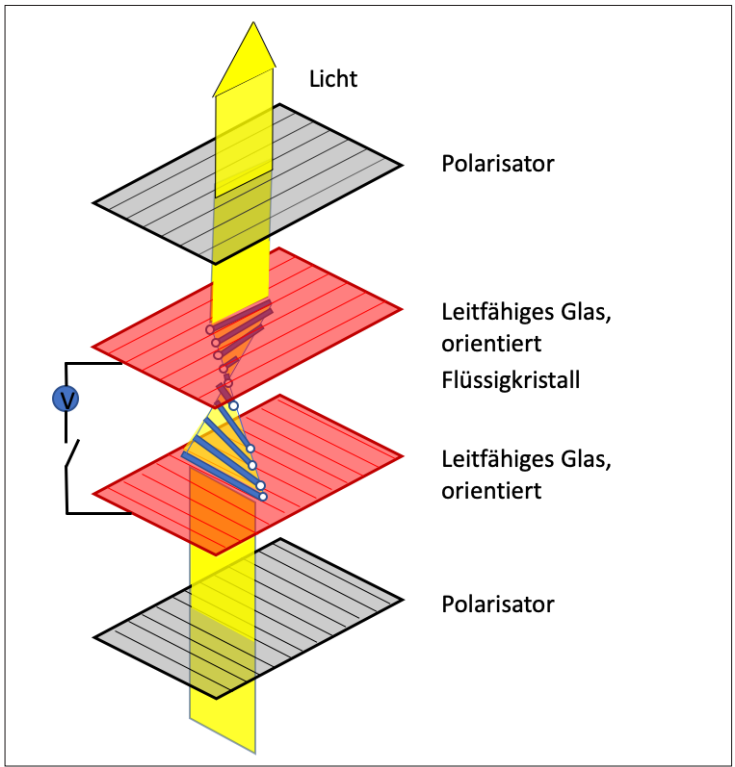
\includegraphics[height=4cm]{pictures/TN-Zelle1.png} & &   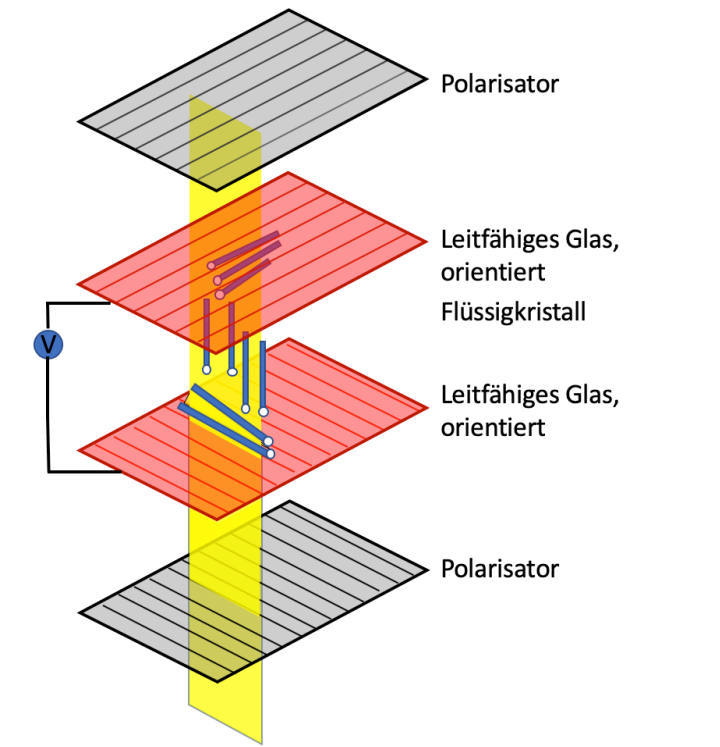
\includegraphics[height=4cm]{pictures/TN-Zelle2.png} \\
        ohne angelegte Spannung  & &  mit angelegter Spannung 
    \end{tabular}
